%\documentclass[justified, twoside, a4paper, symmetric]{tufte-book}
\documentclass{jfp1}

\title{Known When It's Now or Never}

\author{Jos\'{e} Manuel Calder\'{o}n Trilla}


%%%% TODO Package %%%% 
\usepackage[disable,prependcaption,textsize=small]{todonotes}

%\usepackage{amsmath}
\usepackage{xargs}
\usepackage{url}

\usepackage{tikz}
\usepackage{subfig}

\usepackage{csquotes}


\def \hasalpha {\(\alpha\)}
\def \hasbeta {\(\beta\)}
\def \hasgamma {\(\gamma\)}
\def \hasmu {\(\mu\)}
\def \hasphi {\(\phi\)}
\def \haspi {\(\pi\)}
\def \hasrho {\(\rho\)}
\def \haslambda {\(\lambda\)}

\def \meet {\<meet\> ($\sqcap$) }
%\def \pmeet {\bm{\&}}
\def \join {\<join\> ($\sqcup$) }

\newcommandx{\tocite}[2][1=]{\todo[linecolor=red,backgroundcolor=red!25,bordercolor=red,#1]{Cite: #2}}
\newcommandx{\todoinline}[1]{\todo[inline]{#1}}
\newcommandx{\todofig}[1]{\todo[inline]{Make figure: #1}}

\newcommand{\pmeet}{\&}

\usepackage[square]{natbib}

%%%% Haskell Style by Prof. Chakravarty %%%%
\usepackage{haskell}

%This is the stuff for semantic equations%
%%%%%%%%%%%%%%%%%%%%%%%%%%%%%%%%%%%%%%%%%%
\robustify\bfseries
\newsavebox{\sembox}
\newlength{\semwidth}
\newlength{\boxwidth}

\newcommand{\Sem}[1]{%
\sbox{\sembox}{\ensuremath{#1}}%
\settowidth{\semwidth}{\usebox{\sembox}}%
\sbox{\sembox}{\ensuremath{\left[\usebox{\sembox}\right]}}%
\settowidth{\boxwidth}{\usebox{\sembox}}%
\addtolength{\boxwidth}{-\semwidth}%
\left[\hspace{-0.3\boxwidth}%
\usebox{\sembox}%
\hspace{-0.3\boxwidth}\right]%
}
%%%%%%%%%%%%%%%%%%%%%%%%%%%%%%%%%%%%%%%%%%

%% Tikz styles
%%%%%%%%%%%%%%%%%%%%%%%%%%%%%%%%%%%%%%%%%%%%%%%%%%%%%%%%%%%%%%%%%

\tikzset{
    hasse/.style={shape=circle, scale=0.35, draw}
}

\tikzset{
    hassef/.style={fill=black, shape=circle, scale=0.35, draw}
}

\tikzset{
    center/.style={shape=circle, scale=0.35}
}

%% Sometimes we want to give a definition; this is how we do that
%%%%%%%%%%%%%%%%%%%%%%%%%%%%%%%%%%%%%%%%%%%%%%%%%%%%%%%%%%%%%%%%%
\newcommand{\defineword}[2]{%
\begin{description}%
    \item{\textbf{#1}} \hfill \\%
        {#2}%
\end{description}%
}

\newcommand{\sigval}[1]{\bfseries #1}

%%%% hyperref needs to be last (apparently)
%\usepackage{hyperref}
%
%\hypersetup{
% colorlinks,
% citecolor=Red,
% linkcolor=Black,
% urlcolor=Blue
%}


% TODO get this to work with haskell style (figure 26 and 27 especially)
%\usepackage{float} % for box around figures
%\floatstyle{boxed}
%\restylefloat{figure}

% Compromise for the lack of above
%\DeclareCaptionFormat{myformat}{#1#2#3\hrulefill}
%\DeclareCaptionFormat{fnoline}{#1#2#3}
%\captionsetup[figure]{format=myformat}

\begin{document}

\chapter{Finding Safe Parallelism}
\label{chap:discovery} 
Non-strictness makes it difficult to reason about when expressions are
evaluated. This is due to the fact that call-by-need languages only evaluate
expressions when their results are needed, and when a value is needed can
depend on runtime data. One of the benefits of this approach is that it forces
the programmer to avoid the use of arbitrary side-effects. The resulting purity
means that functions in pure functional languages are \emph{referentially
transparent}, or the result of a function depends only on the values of its
arguments (i.e.  there is no global state that could affect the result of the
function or be manipulated by the function).

Unfortunately this elegant evaluation model is actually at odds with the goals
of performance through parallelism: if we have parallel processing resources,
we wish to use them to do as much work as possible to shorten execution time
\citep{tremblay1995impact}.

Call-by-need semantics forces our compiler to take care in deciding which
sub-expressions can safely be executed in parallel. Having a simple
parallelisation heuristic such as `compute all arguments to functions in
parallel' can alter the semantics of a non-strict language, introducing
non-termination or runtime errors that would not have occurred during a
sequential execution.

The process of determining which arguments are required for a function is known
as \emph{strictness analysis} \citep{mycroft1980theory}. Since the early 1980's
such analysis has been widely used for reducing the overheads of lazy
evaluation \citep{SergeyDemand}. As strictness analysis is a form of
termination analysis it is undecidable in general and therefore any results are
approximate. Usually the abstract semantics are chosen so that the analysis can
determine when an expression is \emph{definitely} needed.\footnote{`Needed' in
this context means `needed for the computation to terminate'.}

It is possible to throw caution to the wind and \emph{speculate} on which
expressions may be needed. This itself is a rich area of research and requires
the compiler to identify plausible candidates but ensure that errors and
non-termination do not affect the program as a whole \tocite{speculative 
parallelism work}. For our work we chose to utilise only \emph{safe}
implicit parallelism.

\defineword{Safe Implicit Parallelism}{The parallelism inherent in a program
from tasks/expressions that would have been evaluated during the program's
terminating sequential execution. Any parallelism determined to be safe would not result in
non-termination that was not already present in the program.}

Safe implicit parallelism is in line with our overall goal of providing a system
that guarantees that the parallelised program has the same semantics as the
original. Therefore, before we can run our automatically parallelised programs,
we must develop methods and techniques for the compiler to \emph{find} and
\emph{express} the parallelism that is implicit in our programs. Strictness
analysis is suitable in aiding this task but care must be taken in choosing a
specific analysis to use.

This chapter is concerned with studying the various analyses and the
trade-offs that are inherent in the differing approaches. A survey of the
concepts and development of strictness analysis will inform our choice of
analysis and allow us to understand the drawbacks and limits of our chosen
method.

\subsection*{Plan of the Chapter}

We provide a high-level overview of the issues and motivations in Section
\ref{sec:strictnessOverview}; this should provide enough context to those who
want to move quickly to the next chapter and not concern themselves with the
details of strictness analysis. The ideas are then expanded in the three
sections that follow. Section \ref{sec:twoPoint} explores basic strictness
analysis using the original two-point domain. We will see why a two-point
domain results in an analysis that is too limited for our use in deriving
useful parallel strategies. Using a four-point domain, which we discuss in
Section \ref{sec:fourPoint}, fixes much of this issue and provides much better
information for parallel programs (and has been used toward that end) but does
not allow for analysis on arbitrary data-types. Lastly, we review the work on
projection-based analysis, which solves both issues, in Section
\ref{sec:projections}.


    \section{Original Motivation vs. Our Motivation}
    
Purity alone is of huge benefit when dealing with parallelism. Because
functions do not rely on anything but their arguments, the only necessary communication
between threads is the result of the thread's computation, which is
shared via the program's graph using the same mechanism used to implement
laziness \citep{SPJ:PIFPL}.

Laziness, while forcing the programmer to be pure (a boon to parallelism), is
an inherently sequential evaluation strategy. Lazy evaluation only evaluates
expressions when they are \emph{needed}. This is what allows the use of
infinite data structures; only what is needed will be computed.

This tension between the call-by-need convention of laziness with parallelism's
desire to evaluate expressions \emph{before} they are needed is well known
\citep{tremblay1995impact}. The most successful method of combating this tension
is through the use of \emph{strictness analysis} \citep{mycroft1980theory,
wadler1987projections, hinze1995projection}.


    \section{Overview}
    \label{sec:strictnessOverview}
    Because we are working in a lazy language it is not always safe to evaluate the
arguments to a function before we enter the body of a function. This is easy
to see with a simple example; appending two lists:\footnote{Here we have used
the na\"{i}ve recursive version, but any correct version of append will
have the same strictness properties.}

\begin{haskell*}
append  &::& [\hasalpha] \to [\hasalpha] \to [\hasalpha] \\
append [] ys &=& ys \\
append (x:xs) ys &=& x : append xs ys
\end{haskell*}

\<append\> takes two list arguments. A central question that strictness
analysis asks is: How \emph{defined} must the arguments be to \<append\>
in order for \<append\> to terminate?

The first hint is that \<append\> pattern matches on its first argument.
Because the function must be able to distinguish between a \<(:)\> and a
\<[\ ]\> we know that the first argument must be defined \emph{at least} to
the outermost constructor. Therefore, a use of \<append\> that is passed
$\bot$ as its first argument will result in non-termination. What about the
second argument, \<ys\>. Determining how defined \<ys\> must be turns
out to be impossible without taking into account the \emph{context} that
a call to \<append\> occurs in. If the first argument is \<[\ ]\>
then \<ys\> must be defined to WHNF. However, the \<(:)\> case
guards the recursive call to \<append\> and, by extension, the use
of \<ys\>.

The literature on Strictness Analysis is the story of determining these
properties in the general case. We start in Section \ref{sec:idealAnalysis} with
exploring the simplest strictness analysis, \emph{Ideal Analysis} on \emph{flat
domains}. We then show how the work was extended to \emph{non-flat domains} in
Section \ref{sec:fourPoint}. Lastly, we show how the notion of \emph{contexts}
mentioned above are formalised by the use of \emph{projections} from Domain
Theory in section \ref{sec:projections}.


\subsection{Ideal Strictness Analysis}
\label{sec:idealAnalysis}

If a function uses the value of an argument within its body it is safe
to evaluate that argument before, or in parallel with, the execution of the body
of the function. In order to determine which arguments can be evaluated in this
way modern compilers use \emph{strictness analysis} \citep{mycroft1980theory}.
More formally, a function $f$ of $n$ arguments

$$
    f\ x_{1} \dots \ x_{i} \ \dots x_{n} = \dots
$$

\noindent is strict in its $i$th argument if and only if

$$
    f\ x_{1} \dots \ \bot \ \dots x_{n} = \bot
$$

What this states is that $f$ is only strict in its $i$th argument if $f$
becomes non-terminating\footnote{In this thesis we use the convention that
$\bot$ represents erroneous or non-terminating expressions.} by passing a
non-terminating value as its $i$th argument.

Knowing the strictness information of a function is the first step in automatic
parallelisation. This is because if $f$ is strict in its $i$th argument we do
not risk introducing non-termination (which would not otherwise be present) by
evaluating the $i$th argument in parallel and waiting for the result. In other
words, evaluating $x_{i}$ in parallel would only introduce non-termination to
the program if evaluating $f$ with $x_{i}$ would have resulted in $f$'s
non-termination anyway.

F-Lite has two primitives for taking advantage of strictness information: $par$
and $seq$, as shown in Figure \ref{fig:seqandpar}.
%\begin{figure}
%\begin{tabular}{lll}
%    &seq \ :: \ a \rightarrow b \rightarrow b &&par \ :: \ a \rightarrow b \rightarrow b \\
%    &seq \ x \ y = y                          &&par \ x \ y = y
%\end{tabular}
%\caption[Semantics of \texttt{seq} and \texttt{par}.]{Semantics (but not the pragmatics) of \texttt{seq} and \texttt{par}.}
%\label{fig:seqandpar}
%\end{figure}

Both functions return the value of their second argument. The difference is in
their side-effects. $seq$ returns its second argument only \emph{after}
the evaluation of its first argument. $par$ forks the evaluation of its first
argument in a new parallel thread and then returns its second argument; this is
known as sparking a parallel task \citep{clack1986four}.

Strictness analysis was a very active research area in the 1980's and the
development of analyses that provide the type of strictness information
outlined above is a well understood problem \citep{mycroft1980theory,
clack1985strictness, burn1986strictness}.  However, as suggested above,
strictness analysis does not provide satisfactory information about complex
data-structures \citep{wadler1987strictness}. This can be remedied by the
use of \emph{projections} to represent \emph{demand}.

\subsection{Abstract Interpretation}

Mycroft introduced the use of abstract interpretation for performing strictness
analysis on call-by-need programs over thirty years ago
\citep{mycroft1980theory}.
Strictness analysis as originally described by Mycroft was only capable of
dealing with a two-point domain (values that are definitely needed, and values
that may or may not be needed). This works well for types that can be
represented by a flat domain (Integer, Char, Bool, etc.)\footnote{Any type that
can be represented as an enumerated type.} but falls short on more complex data
structures. For example, even if we find that a function is strict in a list
argument, we can only evaluate up to the first \verb'cons' safely. For many
functions on lists, evaluating the entire list, or the spine of the list, is
safe; canonical examples are \verb'sum' and \verb'length'.

In order to accommodate this type of reasoning, Wadler developed a
\emph{four-point domain} for the abstract interpretation of list-processing
programs \citep{wadler1987strictness}. However, when extended in the natural way
for general recursive data structures, the size of the domains made finding
fix-points prohibitively costly.

\subsection{Projections and Contexts}
\label{sec:projections}

So far our discussion of strictness has only involved two levels of
`definedness': a defined value, or $\bot$. This is the whole story when dealing
with \emph{flat} data-structures such as Integers, Booleans or Enumerations.
However, in lazy languages nested data-structures have \emph{degrees} of
definedness.

Take the following example function and value definitions in F-Lite
\smallskip

\begin{centering}
\begin{verbatim}[commandchars=\\\{\}, codes={\catcode`$=3}]
length []     = 0                   sum []     = 0
length (x:xs) = 1 + length xs       sum (x:xs) = x + sum xs

definedList = [1,2,3,4]             infiniteList = [1,2,3...

partialList = [1,2,$\bot$,4]           loop = loop
\end{verbatim}
\end{centering}

Both \verb-length- and \verb-sum- are functions on lists, but they use lists
differently. \verb-length- does not use the elements of its argument list.
Therefore \verb-length- would accept \verb-definedList- and \verb-partialList-
(which has a non-terminating element) as arguments and still terminate.
On the other hand \verb-sum- \emph{needs} the elements of the list,
otherwise it would not be able to compute the sum. For this reason, \verb-sum-
only terminates if it is passed a fully defined list and would result in
non-termination if passed \verb-partialList-. Neither function would terminate
if passed \verb-infiniteList-, since even \verb-length- requires the list to
have a finite length (some functions do not require a finite list, such as
\verb-head-, the function that returns the first element in a list). With
these examples we say that \verb-length- \emph{demands} a finite list, whereas
\verb-sum- \emph{demands} a fully-defined list.

This additional information about a data-structure is extremely useful when
trying to parallelise programs. If we can determine \emph{how much} of a
structure is needed we can then evaluate the structure to that depth in
parallel.

%The first notable attempt at capturing this type of information was
%by Wadler in 1987 \citep{wadler1987strictness}. However, his approach worked
%well on lists but did not scale well to other, more complex data-structures.

The work that introduced this representation of demands was by Wadler and
Hughes \citep{wadler1987projections} using the idea of \emph{projections} from
domain theory.  The technique we use in our compiler is a projection-based
strictness analysis based on the work in Hinze's dissertation
\citep{hinze1995projection}.  Hinze's dissertation is also a good resource for
learning the theory of projection-based strictness analysis.


\subsection*{Strategies}

With the more sophisticated information provided by projection-based analysis,
we require more than simply $par$ and $seq$ to force the evaluation of values.
To this end we use the popular technique of \emph{strategies} for parallel
evaluation \citep{strategies, marlow2010seq}. Strategies are designed to
evaluate structures up to a certain depth in parallel with the use of those structures. Normally, strategies
are written by the programmer for use in hand-parallelised code. In order to
facilitate auto-parallelisation we have developed a method to \emph{derive} an
appropriate strategy from the information provided to us by projection-based
strictness analysis. The rules for the derivation are presented as a
denotational semantics and will be discussed in Chapter \ref{chap:derivation}.


    \section{Two-Point Forward Analysis}
    \label{sec:twoPoint}
    As mentioned in the Introduction, the majority of functional languages use
either call-by-need or call-by-value semantics.  While call-by-need has many
attractive properties the delaying of computation incurs an overhead cost on
all computations. Call-by-value, by contrast, has an execution model that is
more easily mapped to conventional hardware, allowing for simpler
implementations that achieve good performance. Mycroft used this tension to
motivate his development of strictness analysis \citep{mycroft1980theory}:

\begin{displayquote}

The above arguments suggest that call-by-value is more efficient but
call-by-need preferable on aesthetic/definedness considerations. So techniques
are herein developed which allow the system to present a call-by-need interface
to the user but which performs a pre-pass on his program annotating those
arguments which can validly be passed using call-by-value.

\end{displayquote}

By determining which arguments can be safely passed using call-by-value
we diminish the overhead of call-by-need, paying the overhead of
suspending computation only when necessary to ensure that call-by-need
semantics are maintained.

While this was the original motivation for strictness analysis it also serves
in identifying potential parallelism in a program. When an argument is suitable
to be passed as call-by-value it is also suitable to be evaluated in parallel.
In this case the value is evaluated in parallel to the original thread.
Synchronisation is accomplished via the same mechanism as
laziness,\footnote{Remember that with the spark model of parallelism the
synchronisation occurs via updates to the heap. When a thread begins the
evaluation of an expression it marks the heap node as `locked', stopping any
other thread from repeating the computation.  When the thread completes
evaluation of the expression to WHNF, it updates the locked heap node to point
to the result. Therefore the way threads share computation is identical to the
way a sequential lazy evaluator shares the evaluation of expressions
\citep{clack1986four}.} with the exception that a thread can be blocked while
waiting for another thread to complete its evaluation.

\subsection{Safety First}

Strictness analysis is chiefly concerned with \emph{safety}. In order to retain
the origin call-by-need semantics the runtime can only alter the evaluation order
when doing so guarantees the same termination properties of the program.

We will refer to this notion of safety as the \emph{strictness} properties
of an argument. Take a function $f$ of $n$ arguments

\begin{equation*}
f \ x_{1} \ \dots x_{i} \ \dots \ x_{n} \ = \langle \texttt{function body} \rangle
\end{equation*}

The $i$th argument of $f$ is said to be strict \emph{if and only if}

\begin{equation}
f \ x_{1} \ \dots \bot_{i} \ \dots \ x_{n} \ =  \bot
\end{equation}
\label{eq:idealSafety}

For any possible values of $x_{1}-x_{i-1},x_{i+1}-x_{n}$.

Equation \ref{eq:idealSafety} can be read as ``$f$ is strict in $x_{i}$ when $f$
fails to terminate if $x_{i}$ fails to terminate''. The reason this allows us
to evaluate the $i$th argument before it is needed is because doing so would only result
in introducing non-termination if the program would have resulted in non-termination
otherwise.

\subsection{Abstract Domains}

Now that we have established what it means to be strict we can expand on how we
analyse programs for this property. As with any abstract interpretation,
this involves the choice of an abstract domain.

%% Hasse diagram for the flat domain of integers.
%%
%% We have a horizontal 'number line' from -infity to infinity and edges from each
%% number to _|_ which is centered below the numbers.
\begin{figure}[t]
\centering
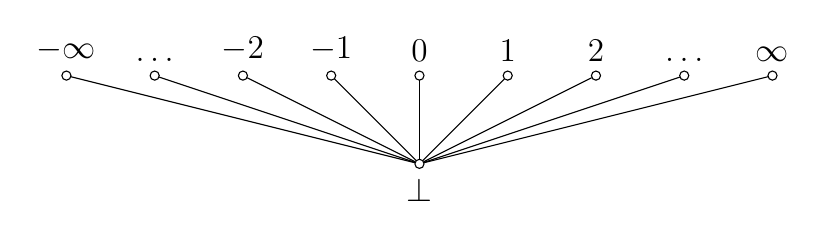
\begin{tikzpicture}
    \node [hasse, label=above:\large$0$]                (zero) at (0,0) {};
    \node [hasse, right = of zero, label=above:\large$1$] (one)   {};
    \node [hasse, right = of one, label=above:\large$2$]  (two)   {};
    \node [hasse, left = of zero, label=above:\large$-1$]  (neg1)  {};
    \node [hasse, left = of neg1, label=above:\large$-2$]  (neg2)  {};
    \node [hasse, left = of neg2, label=above:\large$\dots$]  (ldots) {};
    \node [hasse, right = of two, label=above:\large$\dots$]  (rdots) {};
    \node [hasse, left = of ldots, label=above:\large$-\infty$] (nInf)  {};
    \node [hasse, right = of rdots, label=above:\large$\infty$](inf)   {};

    \node [hasse, below = of zero, label=below:\large$\bot$] (bot)   {};

    \draw[black] (zero) -- (bot);
    \draw[black] (one) -- (bot);
    \draw[black] (two) -- (bot);
    \draw[black] (neg1) -- (bot);
    \draw[black] (neg2) -- (bot);
    \draw[black] (ldots) -- (bot);
    \draw[black] (rdots) -- (bot);
    \draw[black] (inf) -- (bot);
    \draw[black] (nInf) -- (bot);
\end{tikzpicture}
\caption{Flat Domain}
\label{fig:flatInts}
\end{figure}

In non-strict languages types like Integers and Booleans form a flat domain;
either we have a value of that type, or we have $\bot$. This is depicted in
Figure \ref{fig:flatInts}. We can form an intuition of these orderings by
thinking about how much we \emph{know} about a certain value. While the integer
value $5$ maybe greater than the integer value $4$, we know the same amount
about each of them: their values. However, if we have a procedure that is meant
to compute an integer and it loops forever, we cannot know that integer's
value. Therefore we know less about a non-terminating value.


This fits nicely with call-by-need semantics: an argument to a function of
type \<Int\> is really a computation that can either result in a value, or
result in non-termination. In terms of strictness analysis, this allows us to
abstract our real domain of Integers to the simple two-point domain shown in
Figure \ref{fig:twoPointNice}.

\begin{figure}[b]
\centering
\begin{tikzpicture}
    \node [hasse, label=above:\large$\top$]                 (top) {};
    \node [hasse, below = of top, label=below:\large$\bot$] (bot) {};

    \draw[black] (top) -- (bot);
\end{tikzpicture}
\caption{Two-point Domain}
\label{fig:twoPointNice}
\end{figure}


This is the domain we use for basic strictness analysis. The bottom of the
lattice, $\bot$, as implied above, represents \emph{definitely non-terminating}
expressions. The top of the lattice, $\top$, is used to represent
\emph{potentially terminating}\footnote{Remember that program analysis must
approximate in the general case.} expressions. This approximation can seem
counterintuitive; why are we allowing the analysis to say some results are
potentially terminating when they could be non-terminating? The reasoning is
that non-terminating values do not imply a non-terminating program under
non-strict semantics! If we approximated in the opposite direction (as analyses
for other purposes sometimes do) we may accidentally compute a value that was
never needed, defeating the purpose of call-by-need evaluation.


\subsubsection{Abstracting Functions}

Now that we know what it means to be strict and why we represent flat domains
as a two-point domain the next step is to abstract the functions in our
program. 

The idea is simple: for every function in our program of type \<A\> we must
produce a function of type \<A^{\#}\> that works on the abstracted
values.\footnote{Some texts represent an abstracted type by a number \<N\>
where $N$ is the number of points in the abstract domain. We prefer to retain
the context of where this abstract domain came from.} For example, if \<A\> is
the type \<Int \to Int \to Int\>, \<A^{\#}\> would have the abstracted type
\<Int^{\#} \to Int^{\#} \to Int^{\#}\>.  This abstracted program is then
interpreted using an abstract semantics that provides us with the strictness
information for each function in our program.

\begin{figure}[t]
\centering
\begin{minipage}{.5\textwidth}
\begin{haskell*}
\(\top\) \(\sqcap\) \(\top\) &=& \(\top\) \\
\(\top\) \(\sqcap\) \(\bot\) &=& \(\bot\) \\
\(\bot\) \(\sqcap\) \(\top\) &=& \(\bot\) \\
\(\bot\) \(\sqcap\) \(\bot\) &=& \(\bot\)
\end{haskell*}
\end{minipage}
\quad\quad
\begin{minipage}{.5\textwidth}
\begin{haskell*}
\(\top\) \(\sqcup\) \(\top\) &=& \(\top\) \\
\(\top\) \(\sqcup\) \(\bot\) &=& \(\top\) \\
\(\bot\) \(\sqcup\) \(\top\) &=& \(\top\) \\
\(\bot\) \(\sqcup\) \(\bot\) &=& \(\bot\)
\end{haskell*}
\end{minipage}
\caption{The \emph{meet} ($\sqcap$) and \emph{join} ($\sqcup$) for our lattice}
\label{fig:twopointMeet}
\end{figure}

While this separation of abstracting the program and then performing an
abstract interpretation is useful from the theoretical point of view, many
compilers skip the intermediate representation of an abstracted program and
perform the abstract interpretation with the original AST
\citep{hinze1995projection, kubiak, SergeyDemand}.

We begin with the set of primitive arithmetic functions. In the case of F-Lite,
each numeric primitive is strict in both arguments, providing us with the
following for each of \<(+), (-), (*), (/)\>:

\pagebreak

\begin{haskell*}
(\(\odot\)) &::& Int^{\#} \to Int^{\#} \to Int^{\#} \\
\(\top\) \(\odot\) \(\top\) &=& \(\top\) \\
\(\top\) \(\odot\) \(\bot\) &=& \(\bot\) \\
\(\bot\) \(\odot\) \(\top\) &=& \(\bot\) \\
\(\bot\) \(\odot\) \(\bot\) &=& \(\bot\)
\end{haskell*}

We must also be able to combine results from different paths in a program. This
requires both conjunction and disjunction. We can use the \<meet\> ($\sqcap$)
and \<join\> ($\sqcup$) from our lattice which are fully described in Figure
\ref{fig:twopointMeet}.


We can now define an abstract interpretation, $\mathcal{A}$, that takes
expressions in our language and gives us their abstracted values. We require an
environment that maps variables and functions to abstracted values, we use,
\<\hasphi :: Env^{\#}\> to represent this environment. We write
\<\hasphi[x \mapsto v]\> to represent extending the environment with identifier
\<x\> being mapped to the value \<v\>. Lastly, looking up a value in the environment
is just applying the environment to the identifier.

\begin{figure}
\begin{haskell*}
\mathcal{A} &::& Exp \to Env^{\#} \to Exp^{\#} \\
%
\mathcal{A}\Sem{Var v} \hasphi &=& \hasphi v \\
%
\mathcal{A}\Sem{Int i} \hasphi &=& \(\top\) \\
%
\mathcal{A}\Sem{Con c} \hasphi &=& \(\top\) \\
%
\mathcal{A}\Sem{Fun f} \hasphi &=& \hasphi f\\
%
\mathcal{A}\Sem{App (Fun f) [a_{1}, \dots a_{n}]} \hasphi &=&
        \mathcal{A}\Sem{f} \hasphi (\mathcal{A}\Sem{a_{1}} \hasphi) \dots
        (\mathcal{A}\Sem{a_{n}} \hasphi)\\
%
\mathcal{A}\Sem{Let b_{1} = e_{1} \(\dots\) b_{n} = e_{n} in e} \hasphi &=&
        \mathcal{A}\Sem{e} \hasphi[b_{i} \(\mapsto\) \mathcal{A}\Sem{e_{i}}] \\
%
\mathcal{A}\Sem{Case e alts}    \hasphi &=& \mathcal{A}\Sem{e} \hasphi
        \(\sqcap\) \mathcal{C}\Sem{alts} \hasphi \\
%
\quad&\quad&\quad \\
%
\hsnoalign{\mathcal{C}\Sem{c_{1}\ vars_{1} \to e_{n}, \(\dots\), c_{n}\ vars_{n} \to e_{n})} \hasphi =
        e^{\#}_{1} \(\sqcup \dots \sqcup\) e^{\#}_{n}
        \hswhere{%
            e^{\#}_{1} &= \mathcal{A}\Sem{e_{1}} \hasphi[vars_{1} \(\mapsto \top\)] \\
            & \vdots \\
            e^{\#}_{n} &= \mathcal{A}\Sem{e_{n}} \hasphi[vars_{i} \(\mapsto \top\)]
        }
        }
\end{haskell*}
\caption{An Abstract Semantics for Strictness Analysis on a Two-Point Domain}
\label{fig:twoPointAI}
\end{figure}

%\todoinline{Fix rule C so that we take into account the vars introduced by case
%alternatives (they should all be approximated as Top)}

\subsection{Some Examples}

We can now use the abstract semantics from Figure \ref{fig:twoPointAI} on some
real functions.

\subsubsection{The Constant Function:}

The function \<const\> is defined as

\begin{haskell*}
const x y = x
\end{haskell*}

For non-recursive functions, like \<const\>, we can determine the strictness
properties fully with just $n$ iterations of $\mathcal{A}$ where $n$ is the
number of arguments to the function. We run the abstract interpretation using
$\bot$ as the value for the argument we are currently interested in and $\top$
for all the rest.

First we analyse the body (\<x\>) in terms of \<x\>:
\begin{haskell*}
\mathcal{A}\Sem{x}[x \mapsto \(\bot\), y \mapsto \(\top\)] \Rightarrow \(\bot\)
\end{haskell*}

then in terms of \<y\>:
\begin{haskell*}
\mathcal{A}\Sem{x}[x \mapsto \(\top\), y \mapsto \(\bot\)] \Rightarrow \(\top\)
\end{haskell*}

Remembering what it means to be strict from Equation \ref{eq:idealSafety}, this
analysis tells us that \<const\> is strict in \<x\> but not in \<y\>. This is
exactly what we would expect.

\hfill$\Box$

\subsubsection{Conditional}

In non-strict languages we can define our own control-flow abstractions,
allowing what is usually a primitive, the \<if\> statement, to be defined
naturally in the language as

\begin{haskell*}
if p t e = \hscase{p}{\\
                      True \to t\\
                      False \to e}
\end{haskell*}

Analysing \<if\> should determine that \<if\> is strict in \<p\>

\begin{haskell*}
\mathcal{A}\Sem{Case\ p\  [True \to t, False \to e]} \hasphi
\hsbody{%
    \quad& \Rightarrow \mathcal{A}\Sem{p} \hasphi \(\sqcap\)
        (\mathcal{A}\Sem{t} \hasphi \(\sqcup\)
         \mathcal{A}\Sem{e} \hasphi)\\
    \quad& \Rightarrow \(\bot \sqcap (\top \sqcup \top)\)\\
    \quad& \Rightarrow \(\bot\)
}
\hswhere{%
\quad \hasphi = [p \mapsto \(\bot\),t \mapsto \(\top\), e \mapsto \(\top\)]
}
\end{haskell*}

This shows how the use of \<meet\> and \<join\> are used to combine the
results from the different branches of the function. Because the discriminant
of a \<Case\> expression is always evaluated to WHNF, a non-terminating
discriminant results in a non-terminating function.

Notice that if we analysed the second two arguments to \<if\> then we would
have seen that they are not strict for \<if\> because only one would be $\bot$
at a given time and \<meet\> ($\sqcup$) only results in bottom if both arguments
are bottom.


\hfill$\Box$

\subsubsection{Calling Abstract Functions}

Calling functions in the abstract interpretation is the same as a function call
in the standard interpretation except that the target of the call is the
abstracted function. Dependency analysis is used to ensure that callees are
analysed before their callers.\footnote{This also identifies mutually recursive
groups, which we explain next.} The following example illustrates calling
functions and the fact that the abstraction of \<Case\> is capable of
determining when an argument is needed in all the branches.


\begin{haskell*}
addOrConst b x y = \hscase{b}{\\
    True \to x + y\\
    False \to x
    }
\end{haskell*}

The analysis for the second argument proceeds as follows

\begin{haskell*}
\mathcal{A}\Sem{Case\ b\  [True \to x + y, False \to x]} \hasphi
\hsbody{%
    \quad& \Rightarrow \mathcal{A}\Sem{b} \hasphi \(\sqcap\)
        (\mathcal{A}\Sem{x + y} \hasphi \(\sqcup\)
         \mathcal{A}\Sem{x} \hasphi)\\
    \quad& \Rightarrow \(\top\) \(\sqcap\)
        (\mathcal{A}\Sem{x + y} \hasphi \(\sqcup\)
         \mathcal{A}\Sem{x} \hasphi)\\
    \quad& \Rightarrow \(\top\) \(\sqcap\)
        ((\mathcal{A}\Sem{+} \hasphi (\mathcal{A}\Sem{x} \hasphi) (\mathcal{A}\Sem{y} \hasphi)) \(\sqcup\)
         \(\top\))\\
    \quad& \Rightarrow \(\top\) \(\sqcap\)
        ((+^{\#} \(\bot\) \(\top\)) \(\sqcup\)
         \(\top\))\\
    \quad& \Rightarrow \(\top \sqcap (\bot \sqcup \top)\)\\
    \quad& \Rightarrow \(\bot\)
}
\hswhere{%
\quad \hasphi = [b \mapsto \(\top\),x \mapsto \(\bot\), y \mapsto \(\top\)]
}
\end{haskell*}

The other language constructs are interpreted similarly. Do note that we do not
attempt to analyse functions with free variables. Instead we take advantage of
lambda-lifting in order to remove nested functions to the top level. We are not
the first to use lambda lifting in order to avoid this problem
\citep{clack1985strictness}. Luckily, lambda lifting is done regardless for
compilation to the $G$-Machine.

\hfill$\Box$


\subsubsection{Recursive Functions}

Our last concern is with recursive functions. We use the fact that recursive
abstract functions are just recursive functions on a different domain. This
allows us to define a recursive function as the least upper bound of successive
approximations of the function, i.e. an \emph{ascending Kleene chain} (AKC).

We calculate this by starting with the `bottom' approximation where all sets of
inputs are mapped to $\bot$. For a function $f$ we call this $f^{\#0}$. We then
calculate $f^{\#n}$ by replacing each call to $f$ with $f^{\#(n - 1)}$. This
series of successive approximations forms the AKC.

So for a function of the form

\begin{haskell*}
f x_{1} \dots x_{m} = \hsinf{body of \<f\> which includes a call to \<f\>}
\end{haskell*}

We generate the following AKC

\begin{haskell*}
f^{\#0} x_{1} \dots x_{m} &=& \(\bot\) \\
f^{\#1} x_{1} \dots x_{m} &=& \hsinf{body of \<f\> with call to \<f^{\#0}\>} \\
f^{\#2} x_{1} \dots x_{m} &=& \hsinf{body of \<f\> with call to \<f^{\#1}\>} \\
f^{\#3} x_{1} \dots x_{m} &=& \hsinf{body of \<f\> with call to \<f^{\#2}\>} \\
\quad &\vdots& \quad \\
f^{\#n} x_{1} \dots x_{m} &=& \hsinf{body of \<f\> with call to \<f^{\#(n - 1)}\>}
\end{haskell*}

We can stop the calculation of this AKC when $f^{\#n} \equiv f^{\#(n - 1)}$ for
\emph{all combinations} of $x_{1}$ to $x_{m}$. This means that for each iteration
of the AKC we must interpret $f$ $2^m$ times!

Fortunately, there are clever ways of avoiding much of this expense for typical
cases. Clack and Peyton Jones developed an algorithm for the efficient
calculation of an AKC \citep{clack1985strictness}.

\hfill$\Box$

\subsubsection{Discussion of Two-Point Strictness Analysis}

We have now seen how to use semantic function $\mathcal{A}$ from Figure
\ref{fig:twoPointAI} to analyse functions in our programs. Now we can see how
the results help us in our ultimate aim of implicit parallelism. For this
discussion we will forget that parallelism is not always beneficial and focus
on how we would utilise all possible parallelism.

Imagine we have a function $f$ with a call to $g$ in its body.

\begin{haskell*}
f \dots = \dots g e_{1} e_{2} e_{3} \dots
\end{haskell*}

Our analysis may determine that $g$ is strict in its first two arguments,
providing us with an opportunity for parallelism. This would allow us
to safely rewrite $f$ as the following

\begin{haskell*}
f \dots = \dots \hslet{x &= e_{1}\\
                       y &= e_{2}
                       }{%
                       x `par` y `par` g x y e_{3} \dots
                       }
\end{haskell*}

The expressions $e_{1}$ and $e_{2}$ are bound to the names $x$ and $y$
in a \<let\> expression so that the results of parallel evaluation are
shared with the body of $g$.

As mentioned above, the two-point domain informs us about strictness up to
WHNF. So if $e_{1}$ or $e_{2}$ are values from a flat domain, this
transformation will provide all the benefits possible to $g$.\footnote{Again,
ignoring the fact that it may not actually be a positive benefit.} But what if
these arguments are of a non-flat type, like pairs or lists?

Because we aim for safe parallelism, we cannot evaluate $e_{1}$ or $e_{2}$ any
further than WHNF, already eliminating a vast quantity of potential parallelism.
Take the function \<sum\> for example:

\begin{haskell*}
f \dots = \dots \hslet{xs &= e_{1}
                       }{%
                       xs `par` sum xs \dots
                       }
\end{haskell*}

When a programmer wants to express this idiom in their code they often use
\emph{parallel strategies} as illustrated in Section \ref{sec:Approaches}.
This allows the programmer to write an expression similar to \<xs `using`
parList\>. This forces the evaluation of the list beyond WHNF. Because our
two-point domain does not guarantee the safety of evaluating beyond WHNF we are
not able to use a strategy like \<parList\>. This means that even though we
`know' that \<sum\> requires the list fully, the analysis has no way to
represent this, and can only determine that the outermost constructor is
needed!

Because of this shortcoming, strictness analysis in this form is inappropriate
for discovering the parallelism in a program that uses arbitrary algebraic data
structures (e.g. lists or trees). In the next section we will see how this
deficiency is overcome by choosing suitable domains for non-flat structures.

%
%data Exp &=& App Exp [Exp] \\ &|& Case Exp [Alt] \\ &|& Let [Binding] Exp \\
%&|& Fun Id \\


    \section{Four-Point Forward Analysis}
    \label{sec:fourPoint}
    As noted in the last section, two-point domains are quite limited when dealing
with lazy structures. A more formal explanation for this limitation is that the
two-point domain really represents reduction to WHNF or $\bot$, and nothing
else. In the case of flat domains this is sufficient because WHNF is all there
is. For nested data types the reality is much different. 

For functions that work on lists, like \<sum\> or \<append\>, strictness up to
WHNF is not much benefit. Strictness analysis as described in the previous
section would be able to tell us that \<sum\> requires its argument to be
defined, allowing us to evaluate it before entering the function (or in
parallel). But it is only safe up to WHNF. Once the first \<Cons\> is reached
we must stop evaluation of the list or risk introducing non-termination.
Through the lens of implicit parallelism it seems that we are unlikely to
benefit from introducing parallel evaluation when we are limited to
WHNF.\footnote{Indeed most uses of the basic strictness information were for
improving the code generation to avoid building unnecessary suspensions.} This
is clearly a problem.

The solution seems clear: we must extend the abstract domains for non-flat data
types so that we can have more detailed strictness information. For some data
types, extending the technique is straightforward. In F-Lite, pairs can be
defined as follows.

\begin{haskell*}
data Pair \hasalpha \hasbeta = MkPair \hasalpha \hasbeta
\end{haskell*}

Many languages, such as Haskell, Clean, and the ML family provide the following
syntactic sugar for pairs (and other $N$-tuples): \<(\hasalpha,\hasbeta)\>.

A first try at representing pairs of values from the two-point domain could
give us the lattice in Figure \ref{fig:unboxedPairs}.

\begin{figure}
\centering
\subfloat[Unlifted Pairs]{
\begin{tikzpicture}
    \node [center] (cent) {};
    \node [hasse, above = of cent, label=above:{\large\<(\(\top\),\(\top\))\>}]  (top)   {};
    \node [hasse, left = of cent, label=left:{\large\<(\(\top\),\(\bot\))\>}]    (left)  {};
    \node [hasse, right = of cent, label=right:{\large\<(\(\bot\),\(\top\))\>}]  (right) {};
    \node [hasse, below = of cent, label=below:{\large\<(\(\bot\),\(\bot\))\>}] (bot)   {};

    \draw[black] (top) -- (left);
    \draw[black] (top) -- (right);
    \draw[black] (right) -- (bot);
    \draw[black] (left) -- (bot);
\end{tikzpicture}
}
\hfill
\subfloat[Lifted Pairs]{
\begin{tikzpicture}
    \node [center] (cent) {};
    \node [hasse, above = of cent, label=above:{\large\<(\(\top\),\(\top\))\>}]  (top)   {};
    \node [hasse, left = of cent, label=left:{\large\<(\(\top\),\(\bot\))\>}]    (left)  {};
    \node [hasse, right = of cent, label=right:{\large\<(\(\bot\),\(\top\))\>}]  (right) {};
    \node [hasse, below = of cent, label=315:{\large\<(\(\bot\),\(\bot\))\>}] (bot)   {};
    \node [hasse, below = of bot, label=below:{\large$\bot$}] (Bot)   {};

    \draw[black] (top) -- (left);
    \draw[black] (top) -- (right);
    \draw[black] (right) -- (bot);
    \draw[black] (left) -- (bot);
    \draw[black] (bot) -- (Bot);
\end{tikzpicture}
}
\caption{Domain for pairs of flat-domain values}
\hrulefill
\end{figure}

The meaning of this lattice is fairly intuitive. When we possess a pair of
flat-domain values there are four possibilities, we can have

\begin{enumerate}
    \item The pair structure itself (\<MkPair\>), but accessing either value
        results in non-termination
    \item The pair structure itself, but accessing the \<fst\> element 
        results in non-termination
    \item The pair structure itself, but accessing the \<snd\> element
        results in non-termination
    \item The pair structure itself and both values are fully defined
\end{enumerate}

Notice that possibilites 2 and 3 are similar in that there are one defined and
one undefined item in each. Suggesting that one of 2 or 3 is more defined than
the other would make little sense.  For this reason we say that they are
\emph{incomparable}, i.e. they are neither more nor less defined than each
other.

However, the lattice in Figure \ref{fig:unboxedPairs} is only valid for
\emph{unlifted} pairs, where the constructor value, \<(,)\>, is always defined.
The reality for non-strict languages is that \emph{any} value may be undefined,
including the constructors for product types.

This means that we must \emph{lift} the domain, adding a further bottom value
that represents a failure to construct the pair's outermost constructor
(\<MkPair\> in the F-Lite case). The result, shown in Figure
\ref{fig:boxedPairs}, is typical of domains for strictness analysis on finite
types. You can construct an appropriate domain assuming that the structure is
itself defined, then lift the resulting lattice with an additional $\bot$ that
represents a failure to construct the structure.

Because this domain is still finite we are able to incorporate it into the
framework developed by Mycroft without much issue, simply defining the
appropriate \<meet\> and \<join\> on the lattice and the strictness properties
for any primitives that work with pairs. The main issue is that extending the
technique to non-flat domains in the obvious way introduces infinite domains
for recursive types, losing a lot of the power of abstract interpretation.
\tocite{John Hughes work on non-flat domains before wadler and mycroft's thesis
pg 82}

The first practical solution was proposed by Wadler involving a four-point
domain for lists \citep{wadler1987strictness}. Instead of representing the
recursive structure of lists directly, which creates an infinite domain, Wadler
chose a domain that represents four degrees of definedness for lists.

\pagebreak

\begin{figure}[t]
\centering
\begin{tikzpicture}
    \node [hasse, label=above:{\large$\top_{\in}$}]                   (full)   {};
    \node [hasse, below = of full, label=right:{\large$\bot_{\in}$}]  (finite) {};
    \node [hasse, below = of finite, label=right:{\large$\infty$}]    (inf)    {};
    \node [hasse, below = of inf, label=below:{\large$\bot$}]         (bot)    {};

    \draw[black] (full) -- (finite);
    \draw[black] (finite) -- (inf);
    \draw[black] (inf) -- (bot);
\end{tikzpicture}
\caption{Wadler's Four-point Domain}
\label{fig:listDomain}
\end{figure}

The result, as shown in Figure \ref{fig:listDomain}, can be described, from least
to most defined as follows:

\begin{enumerate}
    \item $\bot$ represents all undefined lists
    \item $\infty$ represents all undefined lists, lists  with undefined tails
        and all infinite lists
    \item $\bot_{\in}$ represents all of the above in addition to all finite
        lists with at least one undefined element
    \item $\top_{\in}$ represents fully defined lists along with all of the above
\end{enumerate}


Because we are now concerning ourselves with values from different domains in
our analysis we must now know the types of expressions in our program. This
ensures that we do not accidentally try to \<meet\> or \<join\> values from
different domains. 

\begin{figure}[b]
\centering
\begin{minipage}{.5\textwidth}
\begin{haskell*}
cons^{\#} \(\top\) \(\top_{\in}\) &=& \(\top_{\in}\) \\
cons^{\#} \(\top\) \(\bot_{\in}\) &=& \(\bot_{\in}\) \\
cons^{\#} \(\top\) \(\infty\)     &=& \(\infty\) \\
cons^{\#} \(\top\) \(\bot\)       &=& \(\infty\) \\
\end{haskell*}
\end{minipage}
\quad\quad
\begin{minipage}{.5\textwidth}
\begin{haskell*}
cons^{\#} \(\bot\) \(\top_{\in}\) &=& \(\bot_{\in}\) \\
cons^{\#} \(\bot\) \(\bot_{\in}\) &=& \(\bot_{\in}\) \\
cons^{\#} \(\bot\) \(\infty\)     &=& \(\infty\) \\
cons^{\#} \(\bot\) \(\bot\)       &=& \(\infty\)
\end{haskell*}
\end{minipage}
\caption{Definition of $cons^{\#}$ for a Four-Point Domain}
\label{fig:cons4}
\end{figure}


To incorporate the four-point domain into the abstract interpretation from the
previous section we need a few new primitives. The \<Cons\> constructor is
given the abstract definition shown in Figure \ref{fig:cons4}. \<Nil\>, being a
fully defined list, is always abstracted as $\top_{\in}$.  There are a few
points worth mentioning about the definition of \<cons^{\#}\>.  First, none of
the equations result in $\bot$.  This makes sense with our understanding of
lazy evaluation, if we have the outermost constructor we have a value in WHNF
and therefore it is definitely \emph{not} $\bot$. Additionally, notice that
\<cons\>ing a defined value onto $\bot_{\in}$ also results in $\bot_{\in}$,
this keeps \<cons^{\#}\> monotonic in addition to aligning with our intuitions
(\<cons\>ing a defined element to the beginning of a list with possibly
undefined elements does not suddenly make the list fully defined). 

We must therefore alter the $\mathcal{A}$ rules for nullary constructors and
add a pattern for when \<Cons\> is used. The modified \<Con c\> rule and the
new rule for \<Cons\> are shown in Figure \ref{fig:consAI}.

\begin{figure}[t]
\begin{haskell*}
\mathcal{A}\Sem{Con c} \hasphi && \\
\hsbody{%
    \quad\quad  &\mid c == ``Nil'' &= \(\top_{\in}\) \\
    \quad\quad  &\mid otherwise    &= \(\top\)
    } \\
%
\mathcal{A}\Sem{App (Con ``Cons'') [x, xs]} \hasphi &=&
        cons^{\#} (\mathcal{A}\Sem{x} \hasphi) (\mathcal{A}\Sem{xs} \hasphi)\\
%
\end{haskell*}
\caption{Modification to $\mathcal{A}$ for List Constructors}
\label{fig:consAI}
\end{figure}

In addition to \<Cons\> and \<Nil\>, we need to define new interpretations for
\<Case\> expressions. Pattern matching on a value from the four-point domain
will require a different interpretation than the previous section. The new
domain introduces two problems that must be dealt with:

\begin{enumerate}
    \item Abstracting the alternatives of a \<Case\> expression naively can
        approximate too much, making the results less effective
    \item Choosing appropriate approximations for the bindings introduced with
        the \<Cons\> alternative
\end{enumerate}

We will show the solutions to these obstacles one at a time.

\paragraph{Problem 1:} The first point has to do with pattern matching and
preventing the \<Nil\> alternative from weakening our approximations. For now
we will ignore the question of how to approximate the bindings introduced with
the \<Cons\> alternative.

Take the following template for pattern matching on lists:

\begin{haskell*}
\hscase{\hsinf{a list}}{%
    Nil       &\to \hsinf{\<Nil\> branch} \\
    Cons x xs &\to \hsinf{\<Cons\> branch with possible occurrences of \<x\> and \<xs\>}
    }
\end{haskell*}

If we name the \<Nil\> branch \<a^{\#}\> and treat the \<Cons\> branch as a function
\<f^{\#}\> of \<x\> and \<xs\> we have the following form

\begin{haskell*}
\hscase{\hsinf{a list}}{%
    Nil       &\to a^{\#} \\
    Cons x xs &\to f^{\#} x xs
    }
\end{haskell*}

If we were to naively use the \<Case\> rule from the previous section we
would have\footnote{We use the notation found in \citep{turnerHistory} for
abstracting a variable from an expression: \<[x]e\> denotes abstracting
occurrences of \<x\> out of \<e\>. This results in a function equivalent to
\<(\haslambda x \to e)\>.}

\begin{haskell*}
\mathcal{A}\Sem{Case xs [Nil \to e_{1}, Cons y ys \to e_{2}]} \hasphi &=&
    xs^{\#} \(\sqcap\) (a^{\#} \(\sqcup\) f^{\#} \(\top \ \top_{\in}\))
    \hswhere{%
    &xs^{\#} &= \mathcal{A}\Sem{xs} \hasphi \\
    &a^{\#}  &= \mathcal{A}\Sem{e_{1}} \hasphi \\
    &f^{\#}  &= [ys][y](\mathcal{A}\Sem{e_{2}} \hasphi)
    }
\end{haskell*}

The issue is that the \<meet\>ing of \<a^{\#}\> with \<f^{\#} y ys\> will often
prevent the analysis from providing useful information. Take the function
\<sum\> for example:

\begin{haskell*}
sum xs = \hscase{xs}{%
    Nil       &\to 0 \\
    Cons y ys &\to y + sum ys
    }
\end{haskell*}

In this case, \<a^{\#}\> will always be $\top$, when we abstract the function
to get \<xs^{\#} \(\sqcap\) (\(\top\) \(\sqcup\) f^{\#} y ys)\> the result
would only ever be $\bot$ if \<xs \(\equiv \bot\)\>. Therefore it is only safe
for us to evaluate the list up to WHNF, when \<sum\> clearly needs a
fully-defined list. Moreover, because we may lack information about
the definedness of \<xs\> we must be safe and approximate \<y\> and \<ys\> to
the top of their lattices ($\top$ and $\top_{\in}$, respectively). 

Wadler's key insight was that the use of pattern matching allowed us to retain
information that would otherwise be lost when performing abstract
interpretation \citep{wadler1987strictness}. Whereas in our previous abstract
interpretation from Section \ref{sec:twoPoint} we had to \join all of the
branches in a \<Case\> expression, we can now use the fact that we know \<Nil\>
is always the $\top_{\in}$ value in our domain.  Why is this?  Because \<Nil\>
is a fully defined list with \emph{no bottom elements}!

This means that we only have to consider the value of \<a^{\#}\> when our
\<Case\> expression matches on $\top_{\in}$. This prevents the definedness
of \<a^{\#}\> from preventing more accurate approximations for when the list is
less defined than $\top_{\in}$, solving our first issue.

\paragraph{Problem 2:} The second problem was choosing appropriate approximations
for the bindings introduced with the \<Cons\> alternative. Happily, this turns out
to be quite easy to solve.

In our two-point analysis all bindings introduced by an alternative to a
\<Case\> expression are approximated by $\top$ because we do not `know' how to
approximate non-flat structures. When evaluating a \<Case\> on our four-point
domain we can use the knowledge we have of what lists each point in the domain
corresponds to. We can use the definition of the primitive \<cons^{\#}\> as
a lookup table, switching the right hand and left hand sides of each equation.
This gives us the following:

\begin{haskell}
    \(\top_{\in}\) &\to& cons^{\#} \(\top\) \(\top_{\in}\)              \\  
    \(\bot_{\in}\) &\to& (cons^{\#} \(\bot\) \(\top_{\in}\)) \(\sqcup\)
                         (cons^{\#} \(\top\) \(\bot_{\in}\)) \(\sqcup\)
                         (cons^{\#} \(\bot\) \(\bot_{\in}\)) \(\sqcup\) \\  
    \(\infty\)     &\to& (cons^{\#} \(\top\) \(\infty\))     \(\sqcup\)
                         (cons^{\#} \(\top\) \(\bot\))       \(\sqcup\)
                         (cons^{\#} \(\bot\) \(\infty\))      \(\sqcup\)
                         (cons^{\#} \(\bot\) \(\bot\))
\end{haskell}

The absence of a rule for $\bot$ is due to the fact that we would never match
on an undefined value, resulting in $\bot$ regardless of the values of the
alternatives. We can also remove several of the alternatives in the cases for
$\infty$ and $\bot_{\in}$ due to the necessity for the abstraction of the
alternative branches to be monotonic \citep{wadler1987strictness}.\footnote{For
example, with \(\bot_{\in}\) we will always have \(f^{\#} \bot \bot_{\in}
\sqsubseteq f^{\#} \top \bot_{\in}\), making \(f^{\#} \bot \bot_{\in}\)
unnecessary since \(x \sqcup y \equiv y\) when \(x \sqsubseteq y\). Applying
this reasoning to \(\infty\) leaves us with only \(f^{\#} \top \infty\) to
consider.}

\begin{figure}[t!]
\begin{haskell*}
\mathcal{A}\Sem{Case xs [Nil \to e_{1}, Cons y ys \to e_{2}]} \hasphi && \\
\hsbody{%
    \quad\quad &\mid xs^{\#} == \(\top_{\in}\) &= a^{\#} \(\sqcup\) f^{\#} \(\top\ \top_{\in}\) \\
    \quad\quad &\mid xs^{\#} == \(\bot_{\in}\) &= f^{\#} \(\bot\ \top_{\in}\) \(\sqcup\) f^{\#} \(\top\ \bot_{\in}\) \\
    \quad\quad &\mid xs^{\#} == \(\infty\)     &= f^{\#} \(\top\ \infty\)\\
    \quad\quad &\mid otherwise                 &= \bot
} \hswhere{%
    &xs^{\#} &= \mathcal{A}\Sem{xs} \hasphi \\
    &a^{\#}  &= \mathcal{A}\Sem{e_{1}} \hasphi \\
    &f^{\#}  &= [ys][y](\mathcal{A}\Sem{e_{2}} \hasphi)
    }
\end{haskell*}
\caption{Abstraction of Case Expressions on Lists}
\label{fig:absCase}
\end{figure}


Taking these insights into account leaves us with the rule for
pattern matching on lists seen if Figure \ref{fig:absCase}.

\<meet\> and \<join\> are easily defined for the four-point domain. If we
assign each point in the domain a value according to its position in the lattice,
with $\bot$ being $0$ and $\top_{\in}$ being $3$, we can define \meet as \<min\>
and \join as \<max\>.

With everything in place, we can now determine whether an analysis using this
four-point domain is more suitable for implicit parallelism.

\subsubsection{Length and Sum}

We will use the simple recursive \<length\> function for our first example of
using this analysis (\<sum\> is defined similarly, replacing the \<1\> with
\<y\>).

\begin{haskell*}
length xs &=& \hscase{xs}{%
    Nil &\to 0 \\
    Cons y ys &\to 1 + length ys
    }
\end{haskell*}

Because \<length\> and \<sum\> take only one argument, which is a list, we must
analyse the functions at each of the four points in our domain for lists.
Recursion can be dealt with in the same manner as shown in Section
\ref{sec:twoPoint}. Once a fixed-point is reached we are left with the
following results.

\begin{table}[h!]
\centering
\vspace{10pt}
\begin{tabular}{c || c c}
    $xs^{\#}$ & \<length^{\#} xs^{\#}\> & \<sum^{\#} xs^{\#}\> \\
    \hline
    $\top_{\#}$ & $\top$                & $\top$ \\
    $\bot_{\#}$ & $\top$                & $\bot$ \\
    $\infty$ & $\bot$                   & $\bot$ \\
    $\bot$ & $\bot$                     & $\bot$
\end{tabular}    
\caption{Analysis of \(length^{\#}\) and \(sum^{\#}\) Using 4-point Domains}
\label{tab:lengthSum}
\end{table}

The results in Table \ref{tab:lengthSum} are exactly what we would expect. If
\<length\> or \<sum\> are passed infinite lists then program will result in
non-termination. \<sum\> has the additional constraint that all \emph{elements}
of its input list must also be defined. This analysis would allow us to
evaluate the argument to \<sum\> fully, in parallel, making it a significant
improvement to the simple two-point analysis from Section \ref{sec:twoPoint}.

\subsubsection{Discussion of Four-Point Strictness Analysis}

Because lists are one of the most common structures in functional programming,
this development allowed strictness analysis to be useful in a wide variety of
`real' systems. This also makes strictness analysis' use for parallelism more
realistic. We can now tell the machine to evaluate lists in parallel up to the
degree that it is safe to do so. Some of the more successful attempts at
implicit parallelism were based on using this strictness information, most
notably Burn's work on parallelisation of functional programs for a Spineless
$G$-Machine \citep{burn1987evaluation} and the work of
\citet{hogen1992automatic} on automatically parallelising programs for a
distributed reduction machine.

While this four-point domain made strictness analysis much more flexible it
suffers from a few considerable shortcomings:

\begin{enumerate}
    \item An argument is only considered strict for a function if it is strict
        in \emph{all} possible contexts\footnote{In other words, an argument
                for a function is only strict if it is strict for all possible
                uses of that function. We explore this further in the next
                section.} of that function
    \item For other structures similar domains must be \emph{designed}, i.e.
        there does not seem to be straightforward way to derive a `good' finite
        domain for every recursive type
    \item Even when the compiler writer designs additional abstract domains
        for other recursive types, the calculation of fixed points becomes
        prohibitively expensive with more complex abstract domains
\end{enumerate}

To illustrate the first problem we can study the results of applying this
analysis to the \<append\> function, which can be seen in Table
\ref{tab:append}.

\begin{table}[h!]
\centering
\vspace{10pt}
\begin{tabular}{c c || c c c c}
                               & \multicolumn{1}{c}{} & \multicolumn{4}{c}{$ys^{\#}$}            \\
                               &             & $\top_{\in}$ & $\bot_{\in}$ & $\infty$ & $\bot$   \\
    \cline{2-6}
    \multirow{4}{*}{$xs^{\#}$} & $\top_{\#}$ & $\top_{\in}$ & $\bot_{\in}$ & $\infty$ & $\infty$ \\
                               & $\bot_{\#}$ & $\bot_{\in}$ & $\bot_{\in}$ & $\infty$ & $\infty$ \\
                               & $\infty$    & $\infty$     & $\infty$     & $\infty$ & $\infty$ \\
                               & $\bot$      & $\bot$       & $\bot$       & $\bot$   & $\bot$
\end{tabular}    
\caption{Analysis of \(append^{\#}\ xs^{\#}\ ys^{\#}\) Using 4-point Domains}
\label{tab:append}
\end{table}


We can see that while the first list is always strict up to WHNF, the second
list is not strict. This is unfortunate because we know that \<append\> is
strict in both arguments under certain conditions.

For example, if we pass the result of \<append\> to \<length\> then we know
that \emph{both} argument lists for \<append\> must be finite for the result
of the call the \<length\> to terminate. The inability for this analysis
to express that form of strictness is a major weakness.

The limitations due to this first point were well known at the time of Wadler's
paper on the four-point domain. However, the solutions seemed ad-hoc and were
on shaky theoretical grounds \citep{hughes1986strictness, hughes1987analysing}. The
introduction of the four-point domain was successful, in part, due to it fitting
naturally in the strictness analysis techniques that were already understood.
Fortunately, we have the benefit of time and work on the analysis of strictness that
takes into account the \emph{use} of a function, using \emph{projections}, is
much better understood \citep{hinze1995projection, SergeyDemand}.

The need to design a suitable domain for each recursive type is unfortunate.
Ideally the strictness analysis in a compiler would work on whatever types the
programmer decides to define. Functional languages are often lauded for their
ability to have few primitive types and allow the programmer to define their
own `first class' types.  Having strictness analysis that only functions well
on lists subverts this ideal, creating a leaky abstraction. Programmers will
use lists even when inappropriate because the compiler is so much better at
optimising them than any custom type. While not motivated by the second issue,
projection-based analysis solves it anyway, allowing strictness analysis to be
performed on arbitrary types with very few restrictions.

As for the third shortcoming, projection-based analysis does not make
calculating fixed points free. It does however shift the complexity of the
analysis. Instead of being exponential in the number of arguments, it grows
relative to the size of a function's \emph{return} type. While not a panacea in
this regard it does make projection-based analysis practical.

Overall, strictness analysis using the four-point domain is a significant
improvement over a basic two-point domain, particularly for use in exploiting
implicit parallelism. While having solved several of the downsides of using
a simple two-point domain, the four-point analysis still suffers from
significant problems when taking our use-case into account.


    \section{Projection-Based Analysis}
    \label{sec:projections}
    The shortcomings of the analyses based on the abstract interpretation of
programs motivated Wadler and Hughes to propose using \emph{projections} from
domain theory to analyse strictness \citep{wadler1987projections}.

For our purposes projection-based analysis provides two benefits over abstract
interpretation: simple formulation of domains to analyse functions over
arbitrary structures, and a correspondence with parallel strategies
\citep{marlow2010seq, strategies}. This allows us to use the projections
provided by our analysis to produce an appropriate function to compute the
strict arguments in parallel.

We can frame the differences in the two approaches by thinking about what each
analysis is answering. Strictness analysis by abstract interpretation asks
``When passing $\bot$ as an argument, is the result of the function call
$\bot$?''. Projection-based strictness analysis instead asks ``If there is a
certain degree of demand on the result of this function, what degree of demand
is there on its arguments?''.

What is meant by `demand'? As an example, the function \<length\> requires
that the input list be finite, but no more. We can therefore say that
\<length\> \emph{demands} the spine of the argument list. The function
\<append\> is a more interesting example:

\begin{haskell*}
append &::& [\hasalpha] \to [\hasalpha] \to [\hasalpha] \\
append []     ys &=& ys \\
append (x:xs) ys &=& x : append xs ys
\end{haskell*}

As mentioned in the previous section the first argument must be defined to the
first cons, but we cannot know whether the second argument is ever needed.
However, what if the calling context of \<append\> requires the \emph{result}
of \<append\> to be a finite list?  For example:

\begin{haskell*}
lengthOfBoth &::& [\hasalpha] \to [\hasalpha] \to Int \\
lengthOfBoth xs ys &=& length (append xs ys)
\end{haskell*}

In this case \emph{both} arguments to \<append\> must be finite. Projections
can be used to formalise this type of context \citep{wadler1987projections,
hinze1995projection}, which we call a \emph{demand context}.

\defineword{Demand Context}
           {The depth of a structure that is needed by the consumer of a
            function's result.}

Demand Contexts allow us to reason about the various \emph{uses} of a
function's result, letting us reason about functions like \<append\> more
accurately. This, combined with their ability to analyse functions of arbitrary
types without the need to design abstract domains by hand, make
projection-based analysis the most realistic for our purposes of utilising
implicit parallelism.

\subsection{Semantics of Projections}
\label{sec:projSem}

Given a domain $D$, a projection on $D$ is a continuous function
$\pi \ : \ D \rightarrow D$ that satisfies

\begin{align}
\pi \sqsubseteq ID \\
\pi \circ \pi = \pi
\end{align}

Equation (2) ensures that a projection can not add any information to a value,
i.e. all projections approximate the identity function. Idempotence (3) ensures
that projecting the same demand twice on a value has no additional effect. This
aligns with our intuition of demand. If we demand that a list is spine-strict,
demanding spine-strictness again does not change the demand on the list.

Because we want the introduction of parallelism to be semantics-preserving we
use the following safety condition for projections:

\begin{equation}
\gamma \ \circ \ f = \gamma \ \circ \ f \ \circ \ \pi
\end{equation}

Given a function $f \ : X \rightarrow Y$, and demand $\gamma$ on the
\emph{result} of $f$ we wish to find a safe $\pi$ such that the equality in
Equation (4) remains true. Projection-based analysis propagates the demand
given by $\gamma$ to the arguments of $f$. This results in the demand on the
\emph{arguments} of $f$ given by $\pi$.  The analysis aims to find the
\emph{smallest} $\pi$ for each $\gamma$, but approximating towards $ID$ (as it
is always safe to project the identity).

\paragraph{Demands on Primitives}
On unlifted base types, such as unboxed integers, there are two demands,
$ID$ and $BOT$, with the following semantics


\begin{align}
ID \ x \ &= \ x \\
BOT \ x \ &= \ \bot
\end{align}


When an expression is in a $BOT$ context it means that non-termination is
inevitable. You can safely evaluate an expression in this context because there
is no danger of \emph{introducing} non-termination that is not already present.

\paragraph{Demands on Lifted Types} Haskell's non-strict semantics means that
most types we encounter are \emph{lifted} types.  Lifted types represent
possibly unevaluated values. Given a demand $\pi$ on $D$, we can form two
possible demands on $D_{\bot}$, $\pi!$ and $\pi?$; strict lift and lazy lift
respectively. To paraphrase Kubiak et al.: $\pi!$ means we will definitely need
the value demanded by this projection, and we will need $\pi$'s worth of it
\citep{kubiak}. $\pi?$ does not tell us whether we need the value or not, but if
we \emph{do} need the value, we will need it to satisfy $\pi$'s demand.

\paragraph{Demands on Products} A projection representing a demand on a product
can be formed by using the $\otimes$ operator with the following semantics

\begin{align*}
\langle \pi_{1} \otimes \dots \otimes \pi_{n} \rangle \ \bot &= \bot \\
\langle \pi_{1} \otimes \dots \otimes \pi_{n} \rangle \ 
\langle x_{1}, \dots, x_{n} \rangle &= \langle \pi_{1} x_{1}, \dots, \pi_{n} x_{n} \rangle
\end{align*}

\paragraph{Demands on Sums} If projections are functions on a domain, then
\nolinebreak $|$, the operator that forms projections on sum types performs the
case-analysis. Each summand is tagged with the constructor it corresponds to.
Sometimes we will omit the constructor name when presenting projections on
types with a single summand (such as anonymous tuples).

\begin{align*}
[True\ ID | False\ BOT]  \ True &= True \\
[True\ ID | False\ BOT] \ False &= \bot
\end{align*}

\begin{figure}
\begin{align*}
    \pi ::=&\ BOT              & \text{Bottom (hyperstrict)} \\
        |&\ ID               & \text{Top (the identity)} \\
        |&\ \langle \pi_{1} \otimes \pi_{2} \dots \otimes \pi_{n} \rangle   & \text{Products} \\ 
        |&\ [C_{1} \ \pi_{1} | C_{2} \ \pi_{2} \dots | C_{n} \ \pi_{n}]    & \text{Sums} \\ 
        |&\ \mu\beta . \pi     & \text{Recursive Demands} \\
        |&\ \beta              & \text{Recursive Binding} \\
        |&\ \pi?               & \text{Strict Lift} \\
        |&\ \pi!               & \text{Lazy Lift}
\end{align*}
\caption{Abstract Syntax for Contexts of Demand}
\label{fig:ContextAST}
\end{figure}


Figure \ref{fig:ContextAST} \todo{Add CVars and CRec to AST} presents a
suitable abstract syntax for projections representing demand.  This form was
introduced by Kubiak et al.\ and used in Hinze's work on projection-based
analyses \citep{kubiak, hinze1995projection}.  We have omitted the details on
the representation of context variables (for polymorphic demands). For a
comprehensive discussion we suggest Chapter 6 of Hinze's dissertation
\citep{hinze1995projection}.

In short, projections representing demand give us information about how defined
a value must be to satisfy a function's demand on that value. Knowing that a
value is definitely needed, and to what degree, allows us to evaluate the value
before entering the function.

\subsection*{Example Projections}

Because our primitive values can be modelled by a flat domain (just $ID$ and
$BOT$), our lattice of projections corresponds with the two-point domain used
in abstract interpretation.

\hfill$\Box$

For pairs of primitive values, possible contexts include:
\begin{align}
[\langle ID? \otimes ID? \rangle] \label{IDPairs} \\
[\langle ID! \otimes ID? \rangle] \label{FSTPairs}
\end{align}


As Haskell's types are sums of products, pairs are treated as sums with only
one constructor.  For product types each member of the product is lifted.
Context \ref{IDPairs} is the top of the lattice for pairs, accepting all
possible pairs. Context \ref{FSTPairs} requires that the first member be
defined but does not require the second element. This is the demand that
\<fst\> places on its argument.

\hfill$\Box$

For polymorphic lists there are 7 principal contexts\footnote{All possible
demands on polymorphic lists are instances of one of the 7 principal contexts.}
\citep{hinze1995projection}; 3 commonly occurring contexts are:

\begin{align}
    \mu\beta.&[Nil\ ID | Cons\ \langle \gamma? \otimes \beta?\rangle] \label{IDList} \\
    \mu\beta.&[Nil\ ID | Cons\ \langle \gamma? \otimes \beta!\rangle] \label{FINList} \\
    \mu\beta.&[Nil\ ID | Cons\ \langle \gamma! \otimes \beta!\rangle] \label{FULLList}
\end{align}


Here $\mu$ binds the name for the `recursive call' of the projection and
$\gamma$ is used to represent an appropriate demand for the element type of the
list.  An important point is that this representation for recursive contexts
restricts the representable contexts to \emph{uniform projections}: projections
that define the same degree of evaluation on each of their recursive components
as they do on the structure as a whole. The detailed reason for this
restriction is given on page 89 of \cite{hinze1995projection}. This limitation
does not hinder the analysis significantly as many functions on recursive
structures are themselves uniform.

With this in mind, Context \ref{IDList} represents a lazy demand on the list,
Context \ref{FINList} represents a \emph{tail strict} demand, and Context
\ref{FULLList} represents a \emph{head and tail} strict demand on the list.

\hfill$\Box$

It will be useful to have abbreviations for a few of the contexts on lists. These
abbreviations are presented in Figure \ref{fig:listContexts}.

\begin{figure}[t]
\begin{itemize}
    \item[] \<ID\>: accepts all lists
    \item[] \<T\> (tail strict): accepts all finite lists
    \item[] \<H\> (head strict): accepts lists where the head is defined
    \item[] \<HT\>: accepts finite lists where every member is defined
\end{itemize}
\caption[Projections for the 4-point Domain]{Four contexts on lists as described in \citep{wadler1987projections}.}
\label{fig:listContexts}
\end{figure}

We can now say more about the strictness properties of \<append\>. The
strictness properties of a function are presented as a \emph{context
transformer} \citep{hinze1995projection}. 

\begin{align*}
    &append(ID) &\rightarrow &&ID!&;ID? \\
    &append(T)  &\rightarrow &&T!&;T! \\
    &append(H)  &\rightarrow &&H!&;H? \\
    &append(HT) &\rightarrow &&HT!&;HT!
\end{align*}

This can be read as ``If the demand on the result of \<append\> is $ID$
then the first argument is strict with the demand $ID$ and the second
argument is lazy, but if it \emph{is} needed, it is with demand $ID$.

\hfill$\Box$

Following Hinze \citep{hinze1995projection} we construct projections
for every user-defined type. Each projection represents a
specific strategy for evaluating the structure, as we shall define in section
\ref{sec:derivation}. This provides us with the ability to generate
appropriate parallel strategies for arbitrary types.

\subsection{Lattice of Projections}

Having an intuition  of what projections are we can now define how we combine
differing demands on values. In the previous analyses we used the \meet and
\join operations directly. Projections also have \meet and \join, but because
our projections are representing demand contexts we do not actually want to use
\meet. Instead we use $\pmeet$, where $\alpha\ \pmeet\ \gamma$ represents the
\emph{joint} demand of both $\alpha$'s and $\gamma$'s demand taken together. In
other words, the projection $\alpha\ \pmeet\ \gamma$ only accepts values that
are accepted by $\alpha$ and $\gamma$, and returns $\bot$ otherwise (motivating
the use of `conjunction' to describe the operation). Using $\pmeet$ instead of
$\sqcap$ is standard when dealing with projections that act on demands
\citep{wadler1987projections, hinze1995projection, SergeyDemand}.

Figure \ref{fig:conjDisBasic} shows the rules for performing conjunction and
disjunction of projections on basic values (either $BOT$ or $ID$) and for
lifted values. Note that when we perform $\pmeet$ on two projections with
different lifts we must ensure that the resulting projection is not more strict
than the strictly lifted input, this ensures that we maintain our desired safety
condition.

\begin{figure}
\begin{multicols}{2}
\noindent

\begin{align*}
BOT       &\pmeet  \gamma        &=&\quad BOT \\
\gamma    &\pmeet  BOT           &=&\quad BOT \\
ID        &\pmeet  ID            &=&\quad ID \\
\quad &\             &\ &  \\
\alpha!        &\pmeet  \gamma!  &=&\quad (\alpha \pmeet \gamma)! \\
\alpha!        &\pmeet  \gamma?  &=&\quad (\alpha \sqcup \alpha \pmeet \gamma)! \\
\alpha?        &\pmeet  \gamma!  &=&\quad (\alpha \pmeet \gamma \sqcup \gamma)! \\
\alpha?        &\pmeet  \gamma?  &=&\quad (\alpha \sqcup \gamma)?
\end{align*}% what?

\begin{align*}
BOT            &\sqcup\  \gamma   &=&\quad \gamma \\
\gamma         &\sqcup\  BOT      &=&\quad \gamma \\
ID             &\sqcup\  ID       &=&\quad ID \\
\quad \ \quad  &                  &\ & \\
\alpha!        &\sqcup\  \gamma!  &=&\quad (\alpha \sqcup \gamma)! \\
\alpha!        &\sqcup\  \gamma?  &=&\quad (\alpha \sqcup \gamma)? \\
\alpha?        &\sqcup\  \gamma!  &=&\quad (\alpha \sqcup \gamma)? \\
\alpha?        &\sqcup\  \gamma?  &=&\quad (\alpha \sqcup \gamma)?
\end{align*}
\end{multicols}
\caption[Conjunction and Disjunction for Projections 1]{Conjunction $\pmeet$ and Disjunction $\sqcup$ for Projections on Basic and Lifted Values}
\label{fig:conjDisBasic}
\end{figure}

Figure \ref{fig:conjDisSum} shows the same operations for projections on sum
and product types. The only surprising aspect of the definitions is that we are
forced to normalise the result of a conjunction on product types. This is
because it possible for $\pmeet$ to form a projection denoting $BOT$ even when
both arguments are not $BOT$. For example, applying $\&$ to a projection that
only accepts $True$ and a projection that only accepts $False$ results in the
$BOT$ projection. This is because there is no possible Boolean value that the
resulting projection will accept, despite neither constituent projection
denoting $BOT$.

The \<norm\> function recognises these projections and transforms them to the
direct representation of $BOT$.\footnote{$norm$ is defined in
\cite{hinze1995projection} Section 6.3.}

\subsection{Recursive Types}

\begin{figure}
\noindent

\begin{align*}
[C_{1} \alpha_{1} | \dots | C_{n} \alpha_{n}] \pmeet& [C_{1} \gamma_{1} | \dots | C_{n} \gamma_{n}] \\
    & \quad = [C_{1} (\alpha_{1} \pmeet \gamma_{1}) | \dots | C_{n} (\alpha_{n} \pmeet \gamma_{n})] \\
[C_{1} \alpha_{1} | \dots | C_{n} \alpha_{n}] \sqcup& [C_{1} \gamma_{1} | \dots | C_{n} \gamma_{n}] \\
    & \quad = [C_{1} (\alpha_{1} \sqcup \gamma_{1}) | \dots | C_{n} (\alpha_{n} \sqcup \gamma_{n})]
\end{align*}% what

\begin{align*}
\langle \alpha_{1} \otimes \dots \otimes \alpha_{n} \rangle \pmeet& \langle \gamma_{1} \otimes \dots \otimes \gamma_{n} \rangle \\
    & \quad = norm \big( \langle (\alpha_{1} \pmeet \gamma_{1}) \otimes \dots \otimes (\alpha_{n} \pmeet \gamma_{n})\rangle \big) \\
\langle \alpha_{1} \otimes \dots \otimes \alpha_{n} \rangle \sqcup& \langle \gamma_{1} \otimes \dots \otimes \gamma_{n} \rangle \\
    & \quad = \langle (\alpha_{1} \sqcup \gamma_{1}) \otimes \dots \otimes (\alpha_{n} \sqcup \gamma_{n})\rangle
\end{align*}
\caption[Conjunction and Disjunction for Projections 2]{Conjunction and Disjunction for Projections on Products and Sums}
\label{fig:conjDisSum}
\end{figure}

For conjunction of projections on recursive types we have to perform additional
analysis to ensure that we maintain uniformity, which is the property that the
demand on the `recursive call' of the type is equal to the demand on the type
itself (as mentioned in Section \ref{sec:projSem}). The subtlety is due to the
fact that performing conjunction on two recursive types might result in demands
that differ on the `head' of the value from the demand on the recursive call
\citep{kubiak, hinze1995projection}.

A simple example is when we perform conjunction on the \<H\> and \<T\>
projections on lists (from Figure \ref{fig:listContexts}). If we naively
perform conjunction as
\<(\hasmu\hasbeta.\hasalpha) \pmeet (\hasmu\hasbeta.\hasgamma)
= \hasmu\hasbeta.\hasalpha \pmeet \hasgamma\>, we
arrive at \<HT\>, while this may seem like the correct result it is actually
unsafe! This is clear when applying these projections to the list \<xs = 1 :
\bot : []\>

\pagebreak

\begin{haskell*}
H xs  &\equiv& 1 : \_       &&\hscom{Head strictness forces the first element} \\
T xs  &\equiv& \_ : \_ : [] &&\hscom{Tail strictness forces the spine} \\
HT xs &\equiv& \bot         &&\hscom{\<HT\> forces all elements and the spine}
\end{haskell*}

The reason for the differing results is that \<H\> is not strict in the recursive
part of the list, but \<T\> is, and being head strict is \emph{not} the same
as requiring all elements of a structure, as evidenced by the following small
program

\begin{haskell*}
f xs = a + b \hswhere{%
                a &=&\ head xs \\
                b &=&\ length xs
             }
\end{haskell*}

The demand on the input list \<xs\> is the conjunction of the demands for
\<head\> and \<length\> but it is clear to see that \<f\> does not require its
input list to be fully defined, making it unsafe for \<H \pmeet T\> to result
in \<HT\>.

\hfill$\Box$


The simplest way to maintain uniformity is to take the least upper bound
($\sqcup$) of the two projections.  However, this would be too conservative and
we would lose out on some strictness information that is present. Fortunately,
Hinze provides us with a method that allows us to use more accurate
approximations when it is safe to do so, relying on \join only when necessary
(the last guard in Figure \ref{fig:conjRec}). The idea is to use versions of
$\sqcup$ and $\pmeet$ that ignore all demands except those on the recursive
calls; these are written as $\sqcup'$ and $\pmeet'$. We then see where in the
lattice the result (\<conj\>) resides, performing the corresponding
approximation, defaulting to the always safe \<\hasmu\hasbeta.\hasalpha \sqcup
\hasgamma\>. For details on how this method was derived and a proof of its
safety, see \cite{hinze1995projection} Section 6.4.

\begin{figure}
\begin{haskell*}
(\hasmu\hasbeta.\hasalpha) \sqcup& (\hasmu\hasbeta.\hasgamma) &&= \quad \hasmu\hasbeta.\hasalpha \sqcup \hasgamma &&\ \\
(\hasmu\hasbeta.\hasalpha) \pmeet& (\hasmu\hasbeta.\hasgamma) &&| \quad conj \sqsubseteq \hasbeta_{1} \pmeet' \hasbeta_{2} &&= norm \big(\hasmu\hasbeta.\hasalpha \pmeet \hasgamma \big) \\
\quad                   &   \               &&| \quad conj \sqsubseteq \hasbeta_{1} \sqcup' \hasbeta_{1} \pmeet' \hasbeta_{2} &&= \hasmu\hasbeta.\hasalpha \sqcup \hasalpha \pmeet \hasgamma \\
\quad                   &   \               &&| \quad conj \sqsubseteq \hasbeta_{1} \pmeet' \hasbeta_{2} \sqcup' \hasbeta_{2} &&= \hasmu\hasbeta.\hasalpha \pmeet \hasgamma \sqcup \hasgamma \\
\quad                   &   \               &&| \quad conj \sqsubseteq \hasbeta_{1} \sqcup' \hasbeta_{2} &&= \hasmu\hasbeta.\hasalpha \sqcup \hasgamma
\hswhere{%
    conj &= (norm(\hasalpha[\hasbeta \mapsto \hasbeta_{1}])) \pmeet' (norm(\hasgamma[\hasbeta \mapsto \hasbeta_{2}])) \\
    }
\end{haskell*}
\caption[Conjunction and Disjunction for Projections 3]{Conjunction and Disjuntion for Projections on Recursive Types}
\label{fig:conjRec}
\end{figure}

\subsection{Projection-based Strictness Analysis}

We are now able to present the analysis itself. Being a backward analysis means
that the \emph{result} of our analysis is an environment that maps variables to
demand contexts on those variables. Disjunction and conjunction on these
environments simply performs the operations on the elements in the environment
with the same key. If a key is not present in an environment it is equivalent
to having the lazy demand (top of the demand context lattice for its type).

In order to understand the rules in Figure \ref{fig:projAnal} we must
introduce a few small operators. The $\downarrow$ operator takes a projection on sum types
and a constructor tag and returns the projection corresponding to that constructor:

\begin{haskell*}
[C_{1} \hasalpha_{1} | \dots | C_{i} \hasalpha_{i} | \dots | C_{n} \hasalpha_{n}] \downarrow C_{i} = \hasalpha_{i}
\end{haskell*}

The $\uparrow$ operator performs the dual operation, injecting a projection on
one constructor into a projection on the corresponding sum type. In the
equation below $BOT?$ (also known as the \emph{absent} demand) represents the
lazy lift of the bottom projection for the corresponding sum type:

\begin{haskell*}
C_{i} \uparrow \haspi = [C_{1} BOT? | \dots | C_{i} \haspi | \dots | C_{n} BOT?]
\end{haskell*}

When analysing expressions wrapped in \<Freeze\> we have to be careful because
any demands that originate from suspended values are not \emph{strict} demands.
The \emph{guard} (\<\rhd\>) operator accomplishes this:

\begin{haskell*}
! &\rhd \haspi &= \haspi \\
? &\rhd \haspi &= \haspi \sqcup abs(typeOf(\haspi))
\end{haskell*}

The \<abs(typeOf(\haspi))\> above gets the absent demand for the corresponding
type of the projection \<\haspi\>.

The \<wrap\> and \<unwrap\> functions ensure that we handle recursive types
appropriately. \<unwrap\> is used to `unwrap' the recursive knot one level,
so that

\begin{haskell*}
unwrap \hasalpha@(\hasmu\hasbeta.[Nil \haspi_{1} | Cons \langle \haspi_{2} \otimes \hasbeta_{\ell} \rangle]) =\hsbody{%
    [Nil \haspi_{1} | Cons \langle \haspi_{2} \otimes \hasalpha_{\ell} \rangle]
    }
\end{haskell*}

\<wrap\> is the inverse operation, retying the recursive knot \citep[pg. 117]{hinze1995projection}.

Lastly, \<getProd\> takes a list of identifiers and a projection environment and returns the
projection on the product made up by those identifiers.

\begin{figure}
\begin{haskell*}
\hsnoalign{\mathcal{P} :: Exp \to FunEnv^{\#} \to Context \to Env^{\#}}\\
%
\mathcal{P}\Sem{Var v} \hasphi \haspi &=& \left\{v \mapsto \haspi\right\} \\
%
\mathcal{P}\Sem{Int i} \hasphi \haspi &=& \emptyset \\
%
\mathcal{P}\Sem{Con c} \hasphi \haspi &=& \emptyset \\
%
\mathcal{P}\Sem{Freeze e} \hasphi \haspi_{\ell} &=& \ell \rhd \mathcal{P}\Sem{e} \hasphi \haspi\\
%
\mathcal{P}\Sem{Unfreeze e} \hasphi \haspi &=& \mathcal{P}\Sem{e} \hasphi \haspi! \\
% The hsbody below requires manual spacing... TODO check out why
\mathcal{P}\Sem{App (Con c) as} \hasphi \haspi &\ &
    \hsbody{%
    \quad \quad &\mid null\ as   &= \emptyset \\
    \quad \quad &\mid otherwise  &= overList\ \hasphi\ (unwrap(\haspi) \downarrow c)\ as
    }\\
%
\mathcal{P}\Sem{App (Fun f) as} \hasphi \haspi &\ &
    \hsbody{%
    \quad \quad &\mid null\ as   &= \emptyset \\
    \quad \quad &\mid otherwise  &= overList\ \hasphi\ (\hasphi\ f\ \haspi)\ as
    }\\
%
\mathcal{P}\Sem{Let b = e_{1} in e} \hasphi \haspi &=& env
    \hswhere{%
    \ \hasrho  &= \mathcal{P}\Sem{e} \hasphi \haspi \\
    \ \hasrho' &= \hasrho \setminus \left\{b\right\} \\
    \ env   &= \hskwd{case} lookup b \hasrho \hskwd{of} \hsbody{%
                                    \phantom{env = case lo} Nothing &\to \hasrho' \\
                                    \phantom{env = case lo} Just \hasgamma_{\ell}  &\to \hasrho' \pmeet (\ell \rhd \mathcal{P}\Sem{e_{1}} \hasphi \hasgamma)
                                    }
    }
%
\hsnoalign{\mathcal{P}\Sem{Case\ e\ [C_{1}\ cs_{1} \to e_{1},\ \dots C_{n}\ cs_{n} \to e_{n}]}\ \hasphi\ \haspi
    \hsbody{%
    \phantom{\mathcal{P}\Sem{Let b = e_{1} in e} \hasphi \haspi\ \ \ } &=&\  \hasrho'_{1} \pmeet \mathcal{P}\Sem{e} \hasphi (wrap (C_{1} \uparrow \haspi_{1})) \\
    \          &\ &\  \sqcup \dots \sqcup \\
    \          &\ &\  \hasrho'_{n} \pmeet \mathcal{P}\Sem{e} \hasphi (wrap (C_{n} \uparrow \haspi_{n}))
    \hswhere{%
    \ \hasrho_{1} &=& \mathcal{P}\Sem{e_{1}}\ \hasphi\ \haspi \\
    \ &\vdots & \ \\
    \ \hasrho_{n} &=& \mathcal{P}\Sem{e_{n}}\ \hasphi\ \haspi \\
    \ \quad &\ & \ \\
    \ (\hasrho'_{1}, \haspi_{1}) &=&\ (\hasrho_{1} \setminus cs_{1},\ getProd\ cs_{1}\ \hasrho_{1}) \\
    \ &\vdots & \ \\
    \ (\hasrho'_{n}, \haspi_{n}) &=&\ (\hasrho_{n} \setminus cs_{n},\ getProd\ cs_{n}\ \hasrho_{n})
    }
    }} \\
\end{haskell*}
\caption{Projection-based Strictness Analysis}
\label{fig:projAnal}
\end{figure}


    \section{Summary}
    \label{sec:summ2}
    This chapter explored the most common static analyses used for strictness
analysis.  Because the initial placement of parallelism is crucial to our
technique we explored each possible analysis in depth, highlighting the
drawbacks of the two-point and four-point analyses. While projection-based
analysis is significantly more complex, its ability to determine the strictness
properties of functions based on the \emph{demand} placed on their results
provides too many benefits to ignore.

Many of the previous attempts and using strictness analysis for implicit
parallelism used the four-point analysis. Combined with \emph{evaluation
transformers} (discussed in the next section) the four-point analysis is able
to identify a significant amount of parallelism. Unfortunately, the analysis is
limited to functions on lists, which while ubiquitous, significantly restricts
the potential of identifying parallelism in more complex programs.

The projection-based analysis not only provides more insight into functions
like \<append\>, as discussed in Section \ref{sec:projSem}, but it also allows
us to determine a useful set of strictness properties for functions on
arbitrary types. This greatly expands the applicability of the strictness
analysis for finding potential parallelism.

The major drawback of Hinze's projection-based analysis is that we, as compiler
writers, no longer know in advance the set of demands our analysis will return.
With the four-point analysis we can hard-code the parallel Strategies that
correspond to each of the points in the domain. If we expand our analysis to
include pairs, we can again add the corresponding strategies. With the
projection-based analysis we no longer have that foresight. This is the issue
we address in the next chapter.


% For now we aren't talking about derivin strategies
%
%\chapter{Derivation and Use of Parallel Strategies}
%\label{chap:derivation}
%Non-strictness makes it difficult to reason about when expressions are
evaluated. This is due to the fact that call-by-need languages only evaluate
expressions when their results are needed, and when a value is needed can
depend on runtime data. One of the benefits of this approach is that it forces
the programmer to avoid the use of arbitrary side-effects. The resulting purity
means that functions in pure functional languages are \emph{referentially
transparent}, or the result of a function depends only on the values of its
arguments (i.e.  there is no global state that could affect the result of the
function or be manipulated by the function).

Unfortunately this elegant evaluation model is actually at odds with the goals
of performance through parallelism: if we have parallel processing resources,
we wish to use them to do as much work as possible to shorten execution time
\citep{tremblay1995impact}.

Call-by-need semantics forces our compiler to take care in deciding which
sub-expressions can safely be executed in parallel. Having a simple
parallelisation heuristic such as `compute all arguments to functions in
parallel' can alter the semantics of a non-strict language, introducing
non-termination or runtime errors that would not have occurred during a
sequential execution.

The process of determining which arguments are required for a function is known
as \emph{strictness analysis} \citep{mycroft1980theory}. Since the early 1980's
such analysis has been widely used for reducing the overheads of lazy
evaluation \citep{SergeyDemand}. As strictness analysis is a form of
termination analysis it is undecidable in general and therefore any results are
approximate. Usually the abstract semantics are chosen so that the analysis can
determine when an expression is \emph{definitely} needed.\footnote{`Needed' in
this context means `needed for the computation to terminate'.}

It is possible to throw caution to the wind and \emph{speculate} on which
expressions may be needed. This itself is a rich area of research and requires
the compiler to identify plausible candidates but ensure that errors and
non-termination do not affect the program as a whole \tocite{speculative 
parallelism work}. For our work we chose to utilise only \emph{safe}
implicit parallelism.

\defineword{Safe Implicit Parallelism}{The parallelism inherent in a program
from tasks/expressions that would have been evaluated during the program's
terminating sequential execution. Any parallelism determined to be safe would not result in
non-termination that was not already present in the program.}

Safe implicit parallelism is in line with our overall goal of providing a system
that guarantees that the parallelised program has the same semantics as the
original. Therefore, before we can run our automatically parallelised programs,
we must develop methods and techniques for the compiler to \emph{find} and
\emph{express} the parallelism that is implicit in our programs. Strictness
analysis is suitable in aiding this task but care must be taken in choosing a
specific analysis to use.

This chapter is concerned with studying the various analyses and the
trade-offs that are inherent in the differing approaches. A survey of the
concepts and development of strictness analysis will inform our choice of
analysis and allow us to understand the drawbacks and limits of our chosen
method.

\subsection*{Plan of the Chapter}

We provide a high-level overview of the issues and motivations in Section
\ref{sec:strictnessOverview}; this should provide enough context to those who
want to move quickly to the next chapter and not concern themselves with the
details of strictness analysis. The ideas are then expanded in the three
sections that follow. Section \ref{sec:twoPoint} explores basic strictness
analysis using the original two-point domain. We will see why a two-point
domain results in an analysis that is too limited for our use in deriving
useful parallel strategies. Using a four-point domain, which we discuss in
Section \ref{sec:fourPoint}, fixes much of this issue and provides much better
information for parallel programs (and has been used toward that end) but does
not allow for analysis on arbitrary data-types. Lastly, we review the work on
projection-based analysis, which solves both issues, in Section
\ref{sec:projections}.

%
%    \section{Expressing Need, Strategically}
%    \label{sec:expressingNeed}
%    \input{Deriving-Strats/ExpressingNeed.tex}
%
%    \section{Deriving Strategies from Projections}
%    \label{sec:derivation}
%    \input{Deriving-Strats/StrategyDerivation.tex}
%
%
%    \section{Using Derived Strategies}
%    \label{sec:parPlacement}
%    \input{Platform/Oracles.tex}
    

\bibliography{literature}
\bibliographystyle{jfp}

\end{document}
